% Standalone TikZ diagram: run make in this directory for PDF and SVG.
\documentclass[11pt,tikz,border=2pt]{standalone}
% Shared typography and graph grammar for the L5a standalone TikZ diagrams.
\usepackage{fontspec}
\IfFontExistsTF{Helvetica Neue Light}{
  \setsansfont{Helvetica Neue Light}[BoldFont={Helvetica Neue Medium}]
}{\setsansfont{TeX Gyre Heros}}
\renewcommand{\familydefault}{\sfdefault}
\usepackage{amsmath,amssymb}
\usepackage{unicode-math}
\setmathfont{latinmodern-math.otf}
\usetikzlibrary{arrows.meta,calc,positioning}
\definecolor{vnslideink}{HTML}{333333}
\definecolor{vnslidebody}{HTML}{5E5E5E}
\definecolor{vnaccent}{HTML}{FF644E}
\definecolor{vnslidelink}{HTML}{579ACA}
\definecolor{vnquiet}{HTML}{899198}
\pagecolor{white}
\tikzset{
  every picture/.style={font=\sffamily\small,text=vnslidebody},
  vertex/.style={circle,draw=vnslideink,fill=white,line width=0.7pt,
    minimum size=6.4mm,inner sep=0pt,font=\sffamily\normalsize},
  edge/.style={draw=vnslidebody,line width=0.8pt,
    -{Latex[length=2.2mm,width=1.5mm]},shorten <=3.4mm,shorten >=3.4mm},
  active/.style={edge,draw=vnaccent,line width=1.2pt},
  residual/.style={edge,draw=vnslidelink,line width=1.2pt},
  inactive/.style={edge,draw=vnquiet,line width=0.7pt},
  edge label/.style={fill=white,inner sep=1.4pt,font=\sffamily\small},
  partition/.style={rounded corners=2mm,line width=0.5pt},
}

\begin{document}
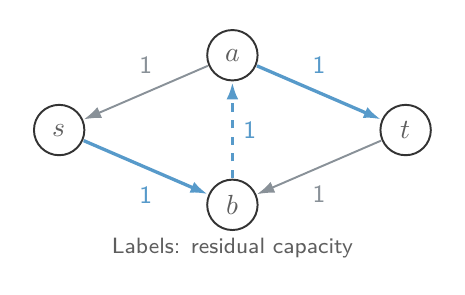
\begin{tikzpicture}[x=1cm,y=1cm]
  \coordinate (s) at (0,0);
  \coordinate (a) at (2.2,0.95);
  \coordinate (b) at (2.2,-0.95);
  \coordinate (t) at (4.4,0);
  \draw[inactive] (a)--node[edge label,above=5pt,text=vnquiet]{1}(s);
  \draw[residual] (s)--node[edge label,below=5pt,text=vnslidelink]{1}(b);
  \draw[residual,dashed] (b)--node[edge label,right=2pt,text=vnslidelink]{1}(a);
  \draw[residual] (a)--node[edge label,above=5pt,text=vnslidelink]{1}(t);
  \draw[inactive] (t)--node[edge label,below=5pt,text=vnquiet]{1}(b);
  \node[font=\sffamily\footnotesize] at (2.2,-1.5) {Labels: residual capacity};
  % Draw nodes after edges so connectors remain behind the vertex disks.
  \foreach \v in {s,a,b,t} {\node[vertex] at (\v) {$\v$};}
  \path[use as bounding box] (-0.4,-1.7) rectangle (4.8,1.3);
\end{tikzpicture}
\end{document}
